% Diagram of the nuclear fuel cycle
% Author: Kathryn Huff
\documentclass[border=10pt]{standalone}
\usepackage{tikz}
\usetikzlibrary{arrows.meta}
\tikzset{%
  >={Latex[width=2mm,length=2mm]},
  % Specifications for style of nodes:
            base/.style = {rectangle, rounded corners, draw=black,
                           minimum width=4cm, minimum height=1cm,
                           text centered, font=\sffamily},
       bluebox/.style = {base, fill=blue!30},
       redbox/.style = {base, fill=red!30},
       greenbox/.style = {base, fill=green!30},
       process/.style = {base, minimum width=2.5cm, fill=orange!15,
                           font=\ttfamily},
}
% Drawing part, node distance is 1.5 cm and every node
% is prefilled with white background
\begin{document}
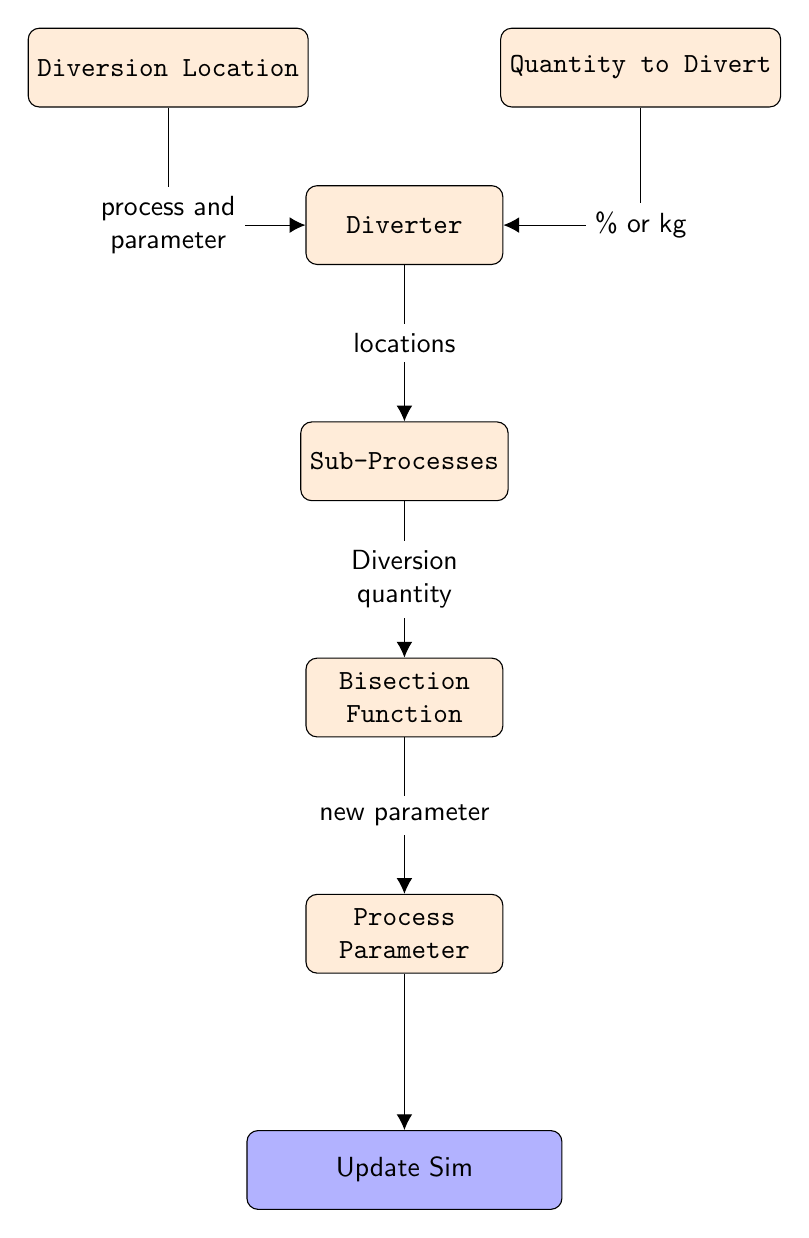
\begin{tikzpicture}[node distance=3cm,
    every node/.style={fill=white, font=\sffamily}, align=center]
  % Specification of nodes (position, etc.)
  \node (top) {};
  \node (location)             [process, left of=top] {Diversion Location};
  \node (quantity)             [process, right of=top] {Quantity to Divert};
  \node (diverter)     [process, below of=top, yshift=1cm]          {Diverter};
  \node (processes)      [process, below of=diverter]   {Sub-Processes};
  \node (eff)     [process, below of=processes]   {Bisection\\Function};
  \node (param)          [process, below of=eff] {Process\\Parameter};
  \node (sim)      [bluebox, below of=param] {Update Sim};
    
  % Specification of lines between nodes specified above
  % with aditional nodes for description 
\draw[->]     (location) |- (diverter) node[midway] {process and\\parameter};
\draw[->]     (quantity) |- (diverter) node[midway] {\% or kg};
\draw[->]     (diverter) -- (processes) node[midway] {locations};
\draw[->]      (processes) -- (eff) node[midway] {Diversion\\quantity};
\draw[->]	  (eff) -- (param) node[midway] {new parameter};
\draw[->]	  (param) -- (sim);


  %\draw[->] (reactor.east) -- ++(2.6,0) -- ++(0,2) -- ++(0,2) --                
  %   node[xshift=1.2cm,yshift=-1.5cm, text width=2.5cm]
  %   {The activity comes to the foreground}(fuelfab.east);
  \end{tikzpicture}
\end{document}

